\chapter{計算実験}\label{computational_result}
\section{計算環境}
実験に用いるプログラムはPythonを用いて実装し, 計算機はMacBookAir2020 (CPU: 8 コア Apple M1 chip, メモリ: 8 GB LPDDR4)を用いて行った. 

\section{第一段階の求解結果}
整数計画ソルバー (Gurobi Optimizer ver. 9.5)を用いて計算した結果, 全ての問題例で最適解が得られた. 
出力の例を図\ref{first-no-rei}に示す. 
長方形内の番号はグループの番号を表す. 
灰色の長方形は, ランプを表す. \\

\begin{figure}[b]
    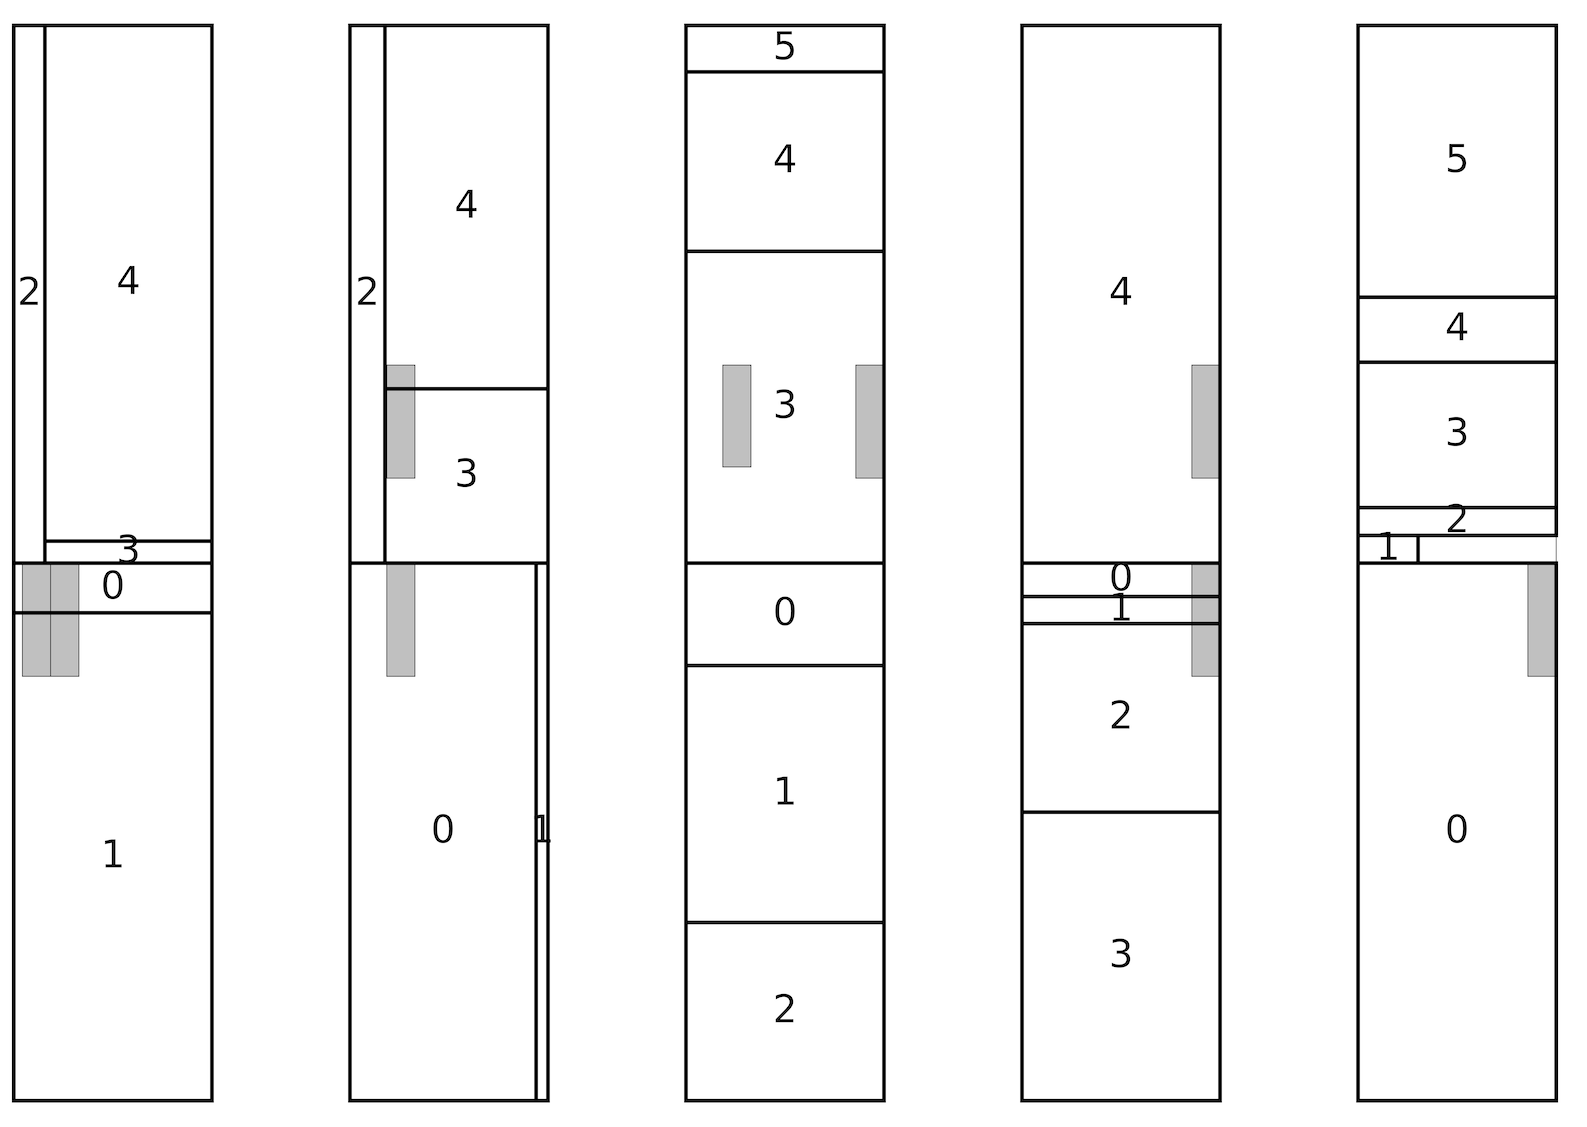
\includegraphics[scale=0.3, bb = 0 0 1 1]{5-first-no-rei.png}
    \caption{第一段階の出力の例}
    \label{first-no-rei}
\end{figure}
\clearpage

\section{第二段階の求解結果}
出力される配置図の例を図\ref{second-no-rei}に示す. 
各長方形が車を表し, 色は揚げ地の種類を表す. \\

\begin{figure}[b]
    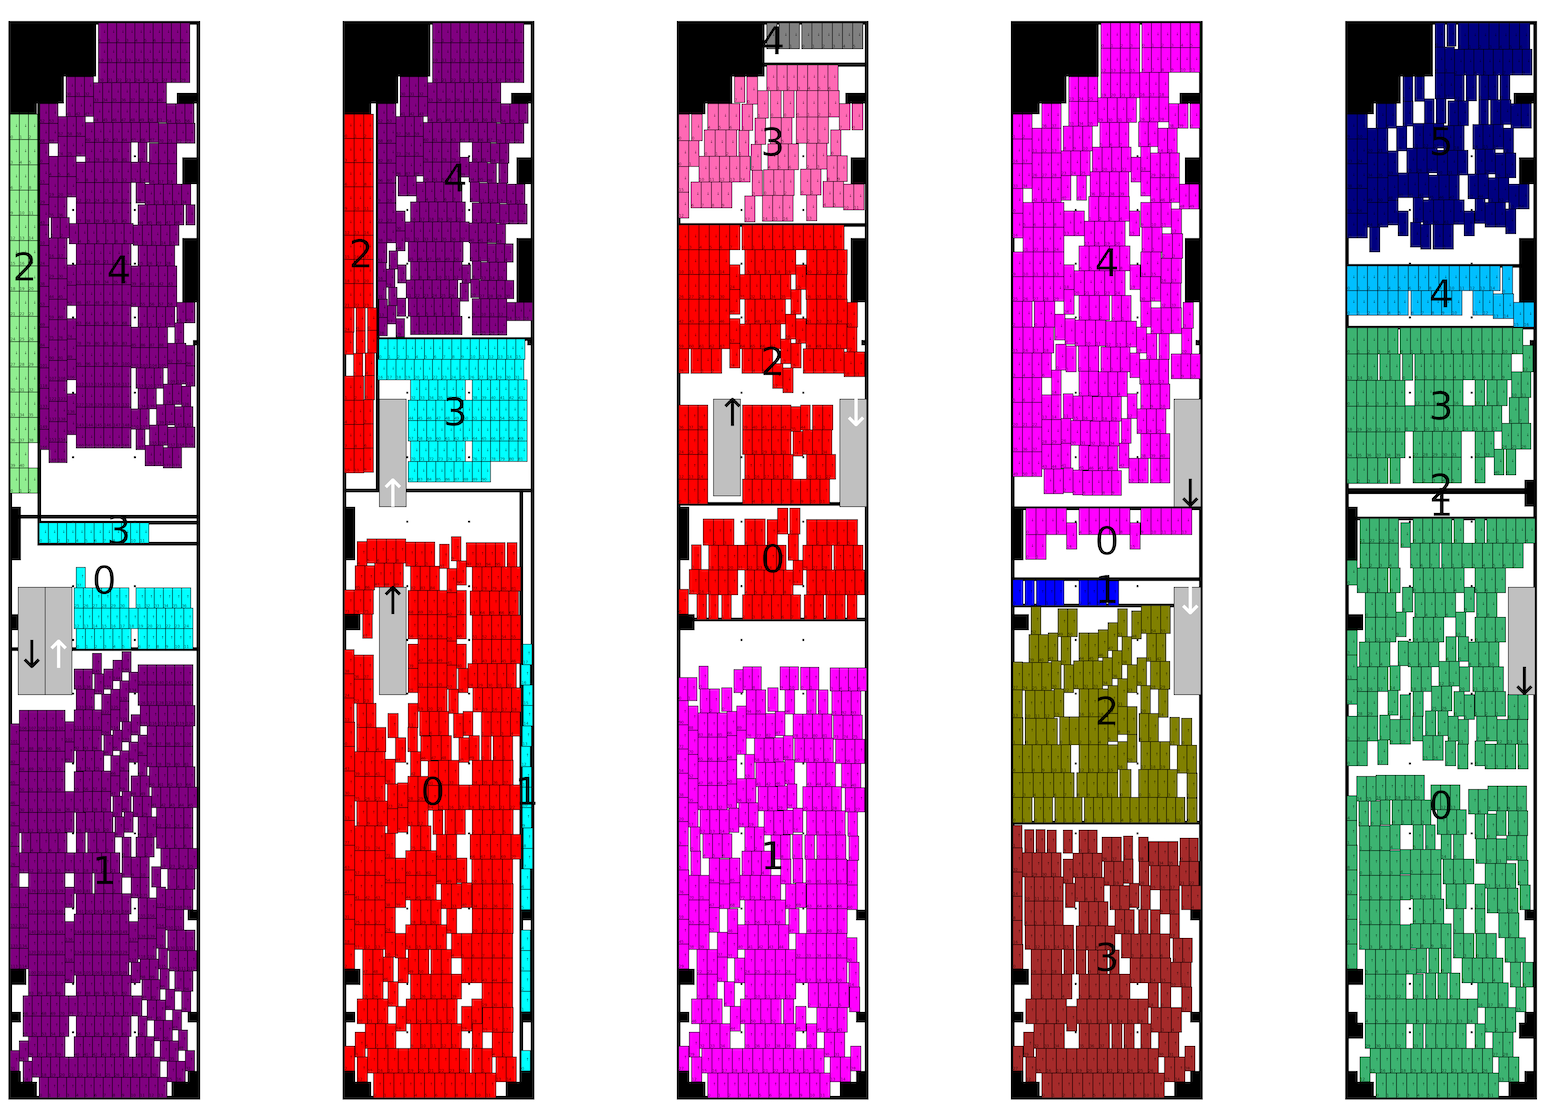
\includegraphics[scale=0.3, bb = 0 0 1 1]{5-second-no-rei.png}
    \caption{第二段階の出力図の例}
    \label{second-no-rei}
\end{figure}

\section{局所探索法による解の改善}
表\ref{review-local}に初期解生成による結果と局所探索を加えた手法の結果を示す. 
表の余りの台数, はデッキに詰め込むことのできなかった車の台数を表す. 
デッキの面積から障害物の総面積を引いたものを配置可能面積とし, 配置可能面積における配置した車の総面積の割合を充填率として表す. 


\begin{landscape}    
\begin{table}[p]
    \caption{近傍操作による解の改善}
    \label{review-local}
    \begin{tabular}{cccccclccc}
    \hline
    \multicolumn{2}{c}{問題例} &  & \multicolumn{3}{c}{初期解生成のみ}     &  & \multicolumn{3}{c}{局所探索あり}      \\
    \hline
    問題番号      & 詰め込む台数      &  & 余りの台数 (台) & 計算時間 (s) & 充填率 (\%) &  & 余りの台数 (台) & 計算時間 (s) & 充填率 (\%) \\
    \hline
    1         & 773         &  & 20        & 75       & 75.7     &  & 7         & 647      & 77.0     \\
    2         & 691         &  & 200       & 95       & 76.6     &  & 18        & 390      & 76.6     \\
    3         & 585         &  & 27        & 116      & 73.7     &  & 27        & 419      & 73.7     \\
    4         & 604         &  & 91        & 174      & 68.3     &  & 44        & 663      & 74.3     \\
    5         & 594         &  & 35        & 196      & 74.8     &  & 27        & 619      & 76.0     \\
    6         & 481         &  & 17        & 143      & 68.3     &  & 5         & 776      & 70.1     \\
    7         & 370         &  & 3         & 101      & 54.5     &  & 3         & 470      & 54.5     \\
    8         & 530         &  & 10        & 178      & 77.6     &  & 10        & 607      & 77.6     \\
    9         & 545         &  & 92        & 157      & 66.4     &  & 92        & 579      & 66.4     \\
    10        & 581         &  & 91        & 178      & 66.5     &  & 91        & 607      & 66.5     \\
    11        & 530         &  & 6         & 174      & 74.3     &  & 6         & 498      & 74.3     \\
    12        & 641         &  & 26        & 184      & 75.5     &  & 26        & 502      & 75.5     \\
    13        & 609         &  & 88        & 95       & 65.5     &  & 88        & 247      & 65.5     \\
    14        & 675         &  & 72        & 165      & 67.6     &  & 72        & 491      & 67.6     \\
    15        & 629         &  & 1         & 193      & 80.2     &  & 1         & 664      & 80.2     \\
    \hline
    \end{tabular}
\end{table}
\end{landscape}